\documentclass[11pt,]{article}
\usepackage[left=1in,top=1in,right=1in,bottom=1in]{geometry}
\newcommand*{\authorfont}{\fontfamily{phv}\selectfont}
\usepackage[]{mathpazo}


  \usepackage[T1]{fontenc}
  \usepackage[utf8]{inputenc}




\usepackage{abstract}
\renewcommand{\abstractname}{}    % clear the title
\renewcommand{\absnamepos}{empty} % originally center

\renewenvironment{abstract}
 {{%
    \setlength{\leftmargin}{0mm}
    \setlength{\rightmargin}{\leftmargin}%
  }%
  \relax}
 {\endlist}

\makeatletter
\def\@maketitle{%
  \newpage
%  \null
%  \vskip 2em%
%  \begin{center}%
  \let \footnote \thanks
    {\fontsize{18}{20}\selectfont\raggedright  \setlength{\parindent}{0pt} \@title \par}%
}
%\fi
\makeatother




\setcounter{secnumdepth}{0}

\usepackage{color}
\usepackage{fancyvrb}
\newcommand{\VerbBar}{|}
\newcommand{\VERB}{\Verb[commandchars=\\\{\}]}
\DefineVerbatimEnvironment{Highlighting}{Verbatim}{commandchars=\\\{\}}
% Add ',fontsize=\small' for more characters per line
\usepackage{framed}
\definecolor{shadecolor}{RGB}{248,248,248}
\newenvironment{Shaded}{\begin{snugshade}}{\end{snugshade}}
\newcommand{\AlertTok}[1]{\textcolor[rgb]{0.94,0.16,0.16}{#1}}
\newcommand{\AnnotationTok}[1]{\textcolor[rgb]{0.56,0.35,0.01}{\textbf{\textit{#1}}}}
\newcommand{\AttributeTok}[1]{\textcolor[rgb]{0.77,0.63,0.00}{#1}}
\newcommand{\BaseNTok}[1]{\textcolor[rgb]{0.00,0.00,0.81}{#1}}
\newcommand{\BuiltInTok}[1]{#1}
\newcommand{\CharTok}[1]{\textcolor[rgb]{0.31,0.60,0.02}{#1}}
\newcommand{\CommentTok}[1]{\textcolor[rgb]{0.56,0.35,0.01}{\textit{#1}}}
\newcommand{\CommentVarTok}[1]{\textcolor[rgb]{0.56,0.35,0.01}{\textbf{\textit{#1}}}}
\newcommand{\ConstantTok}[1]{\textcolor[rgb]{0.00,0.00,0.00}{#1}}
\newcommand{\ControlFlowTok}[1]{\textcolor[rgb]{0.13,0.29,0.53}{\textbf{#1}}}
\newcommand{\DataTypeTok}[1]{\textcolor[rgb]{0.13,0.29,0.53}{#1}}
\newcommand{\DecValTok}[1]{\textcolor[rgb]{0.00,0.00,0.81}{#1}}
\newcommand{\DocumentationTok}[1]{\textcolor[rgb]{0.56,0.35,0.01}{\textbf{\textit{#1}}}}
\newcommand{\ErrorTok}[1]{\textcolor[rgb]{0.64,0.00,0.00}{\textbf{#1}}}
\newcommand{\ExtensionTok}[1]{#1}
\newcommand{\FloatTok}[1]{\textcolor[rgb]{0.00,0.00,0.81}{#1}}
\newcommand{\FunctionTok}[1]{\textcolor[rgb]{0.00,0.00,0.00}{#1}}
\newcommand{\ImportTok}[1]{#1}
\newcommand{\InformationTok}[1]{\textcolor[rgb]{0.56,0.35,0.01}{\textbf{\textit{#1}}}}
\newcommand{\KeywordTok}[1]{\textcolor[rgb]{0.13,0.29,0.53}{\textbf{#1}}}
\newcommand{\NormalTok}[1]{#1}
\newcommand{\OperatorTok}[1]{\textcolor[rgb]{0.81,0.36,0.00}{\textbf{#1}}}
\newcommand{\OtherTok}[1]{\textcolor[rgb]{0.56,0.35,0.01}{#1}}
\newcommand{\PreprocessorTok}[1]{\textcolor[rgb]{0.56,0.35,0.01}{\textit{#1}}}
\newcommand{\RegionMarkerTok}[1]{#1}
\newcommand{\SpecialCharTok}[1]{\textcolor[rgb]{0.00,0.00,0.00}{#1}}
\newcommand{\SpecialStringTok}[1]{\textcolor[rgb]{0.31,0.60,0.02}{#1}}
\newcommand{\StringTok}[1]{\textcolor[rgb]{0.31,0.60,0.02}{#1}}
\newcommand{\VariableTok}[1]{\textcolor[rgb]{0.00,0.00,0.00}{#1}}
\newcommand{\VerbatimStringTok}[1]{\textcolor[rgb]{0.31,0.60,0.02}{#1}}
\newcommand{\WarningTok}[1]{\textcolor[rgb]{0.56,0.35,0.01}{\textbf{\textit{#1}}}}

\usepackage{graphicx,grffile}
\makeatletter
\def\maxwidth{\ifdim\Gin@nat@width>\linewidth\linewidth\else\Gin@nat@width\fi}
\def\maxheight{\ifdim\Gin@nat@height>\textheight\textheight\else\Gin@nat@height\fi}
\makeatother
% Scale images if necessary, so that they will not overflow the page
% margins by default, and it is still possible to overwrite the defaults
% using explicit options in \includegraphics[width, height, ...]{}
\setkeys{Gin}{width=\maxwidth,height=\maxheight,keepaspectratio}


\title{Programación Estadística: Ascenso a la cordillera  }



\author{\Large Adrián Sosa\vspace{0.05in} \newline\normalsize\emph{}   \and \Large \vspace{0.05in} \newline\normalsize\emph{Universidad Veracruzana}  }



\date{}

\usepackage{titlesec}

\titleformat*{\section}{\normalsize\bfseries}
\titleformat*{\subsection}{\normalsize\itshape}
\titleformat*{\subsubsection}{\normalsize\itshape}
\titleformat*{\paragraph}{\normalsize\itshape}
\titleformat*{\subparagraph}{\normalsize\itshape}


\usepackage{natbib}
\bibliographystyle{plainnat}
\usepackage[strings]{underscore} % protect underscores in most circumstances



\newtheorem{hypothesis}{Hypothesis}
\usepackage{setspace}


% set default figure placement to htbp
\makeatletter
\def\fps@figure{htbp}
\makeatother

\usepackage{hyperref}

% move the hyperref stuff down here, after header-includes, to allow for - \usepackage{hyperref}

\makeatletter
\@ifpackageloaded{hyperref}{}{%
\ifxetex
  \PassOptionsToPackage{hyphens}{url}\usepackage[setpagesize=false, % page size defined by xetex
              unicode=false, % unicode breaks when used with xetex
              xetex]{hyperref}
\else
  \PassOptionsToPackage{hyphens}{url}\usepackage[draft,unicode=true]{hyperref}
\fi
}

\@ifpackageloaded{color}{
    \PassOptionsToPackage{usenames,dvipsnames}{color}
}{%
    \usepackage[usenames,dvipsnames]{color}
}
\makeatother
\hypersetup{breaklinks=true,
            bookmarks=true,
            pdfauthor={Adrián Sosa () and  (Universidad Veracruzana)},
            pdfkeywords = {},  
            pdftitle={Programación Estadística: Ascenso a la cordillera},
            colorlinks=true,
            citecolor=blue,
            urlcolor=blue,
            linkcolor=magenta,
            pdfborder={0 0 0}}
\urlstyle{same}  % don't use monospace font for urls

% Add an option for endnotes. -----


% add tightlist ----------
\providecommand{\tightlist}{%
\setlength{\itemsep}{0pt}\setlength{\parskip}{0pt}}

% add some other packages ----------

% \usepackage{multicol}
% This should regulate where figures float
% See: https://tex.stackexchange.com/questions/2275/keeping-tables-figures-close-to-where-they-are-mentioned
\usepackage[section]{placeins}


\begin{document}
	
% \pagenumbering{arabic}% resets `page` counter to 1 
%
% \maketitle

{% \usefont{T1}{pnc}{m}{n}
\setlength{\parindent}{0pt}
\thispagestyle{plain}
{\fontsize{18}{20}\selectfont\raggedright 
\maketitle  % title \par  

}

{
   \vskip 13.5pt\relax \normalsize\fontsize{11}{12} 
\textbf{\authorfont Adrián Sosa} \hskip 15pt \emph{\small }   \par \textbf{\authorfont } \hskip 15pt \emph{\small Universidad Veracruzana}   
}

}






\vskip -8.5pt


 % removetitleabstract

\noindent  

\hypertarget{ascenso-a-la-cordillera}{%
\subsection{Ascenso a la cordillera}\label{ascenso-a-la-cordillera}}

El asenso a la colina es un método simple de optimización local que
``sube'' la colina hasta se encuentra un óptimo local (asumiendo una
meta de maximización). El método funciona mediante la búsqueda iterativa
de nuevas soluciones dentro del entorno de las soluciones, adoptando
nuevas soluciones si son mejores, como se muestra en el pseudocódigo del
algoritmo. El propósito del cambio de función es producir una solución,
realizando una búsqueda completa en todo el vecindario o aplicando un
pequeño cambio aleatorio en los valores de la solución actual. Cabe
señalar que si bien el el algoritmo estándar de escalada es
determinista, cuando se utilizan cambios aleatorios paros perturbando
una solución, se logra un comportamiento estocástico. Por esta razón en
ascenso a la colina es situado en el medio de la dimensión determinista
/ estocástica. Hay varias variantes de escalada, como la escalada más
empinada

\hypertarget{ventajas}{%
\subsubsection{Ventajas}\label{ventajas}}

\begin{itemize}
\tightlist
\item
  Reduce el número de nodos a analizar
\end{itemize}

\hypertarget{desventajas}{%
\subsubsection{Desventajas}\label{desventajas}}

\begin{itemize}
\tightlist
\item
  Puede ser que encuentre una solución, pero no sea la más óptima
\end{itemize}

\hypertarget{pseudocuxf3digo}{%
\subsubsection{PSEUDOCÓDIGO}\label{pseudocuxf3digo}}

\emph{Selección:} empezar desde la raíz \emph{R} y seleccionar nodos
hijos sucesivos hasta alcanzar un nodo hoja \emph{L}. La selección
describe una manera de elegir los nodos hijos, que permitan que el árbol
se expanda hacia movimientos mas prometedores, que es la esencia del
árbol de búsqueda Monte Carlo.

\begin{figure}
\centering
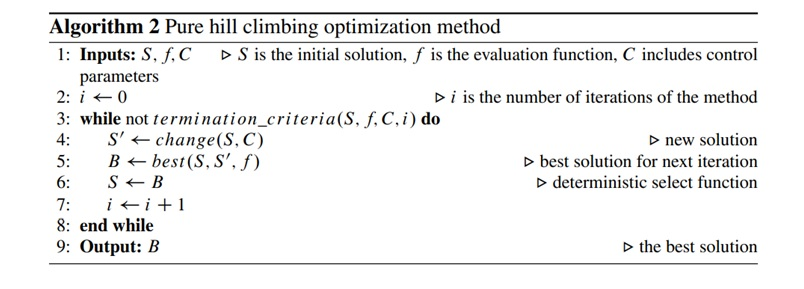
\includegraphics{./imagenes/pseudocodigo.jpg}
\caption{Pseudocódigo}
\end{figure}

\newpage

\hypertarget{codificaciuxf3n}{%
\subsubsection{Codificación}\label{codificaciuxf3n}}

La codificación de Búsqueda Monte Carlo es relativamente sencilla, al
hacer uso de el método de búsqueda ciega:

\begin{Shaded}
\begin{Highlighting}[]
\NormalTok{hclimbing}
\end{Highlighting}
\end{Shaded}

\begin{verbatim}
## function (x, Fx, lower, upper, type = "min", N = 1000, ...) 
## {
##     D <- length(lower)
##     s <- matrix(nrow = N, ncol = D)
##     for (i in 1:N) s[i, ] = runif(D, lower, upper)
##     best <- fsearch(sol = s, Fx = Fx, type = type, ...)
##     best_1 <- Fx(x, ...)
##     if (type == "min") {
##         if (best_1 < best$eval) 
##             return(list(sol = x, eval = best_1))
##         else hclimbing(best$sol, Fx, lower, upper, type, N, ...)
##     }
##     else {
##         if (best_1 > best$eval) 
##             return(list(sol = x, eval = best_1))
##         else hclimbing(best$sol, Fx, lower, upper, type, N, ...)
##     }
## }
\end{verbatim}

Su implementación de igual manera es sencilla:

\begin{Shaded}
\begin{Highlighting}[]
\NormalTok{N=}\DecValTok{10000}                              \CommentTok{# se define el número de muestras}
\NormalTok{limI <-}\StringTok{ }\DecValTok{-5}
\NormalTok{limS <-}\StringTok{ }\DecValTok{5}
\NormalTok{var <-}\StringTok{ }\DecValTok{1}                                       \CommentTok{# número de variables}
\NormalTok{upper <-}\StringTok{ }\KeywordTok{rep}\NormalTok{ (limS,var)                }\CommentTok{# vector con el valor mas alto de cada dimensión}
\NormalTok{lower <-}\StringTok{ }\KeywordTok{rep}\NormalTok{ (limI,var)                }\CommentTok{# vector con el valor mas bajo de cada dimensión}
\NormalTok{x <-}\StringTok{ }\DecValTok{1}                             \CommentTok{# punto inicial}

\NormalTok{fx <-}\StringTok{ }\NormalTok{rastrigin}
\NormalTok{label <-}\StringTok{ "Rastrigin: "}
\NormalTok{min <-}\StringTok{ }\KeywordTok{hclimbing}\NormalTok{(x,fx,lower,upper,}\DataTypeTok{type=}\StringTok{"min"}\NormalTok{)}
\NormalTok{max <-}\StringTok{ }\KeywordTok{hclimbing}\NormalTok{(x,fx,lower,upper,}\DataTypeTok{type=}\StringTok{"max"}\NormalTok{)}

\KeywordTok{cat}\NormalTok{(}\KeywordTok{c}\NormalTok{(label, }\StringTok{"Solución mínima: "}\NormalTok{, min}\OperatorTok{$}\NormalTok{sol,}\StringTok{" Evaluación: "}\NormalTok{, min}\OperatorTok{$}\NormalTok{eval,}\StringTok{"}\CharTok{\textbackslash{}n}\StringTok{"}\NormalTok{))}
\end{Highlighting}
\end{Shaded}

\begin{verbatim}
## Rastrigin:  Solución mínima:  -0.00150685897096992  Evaluación:  0.000450470480126697
\end{verbatim}

\begin{Shaded}
\begin{Highlighting}[]
\KeywordTok{cat}\NormalTok{(}\KeywordTok{c}\NormalTok{(label, }\StringTok{"Solución máxima: "}\NormalTok{, max}\OperatorTok{$}\NormalTok{sol,}\StringTok{" Evaluación: "}\NormalTok{, max}\OperatorTok{$}\NormalTok{eval,}\StringTok{"}\CharTok{\textbackslash{}n}\StringTok{"}\NormalTok{))}
\end{Highlighting}
\end{Shaded}

\begin{verbatim}
## Rastrigin:  Solución máxima:  -4.52048848383129  Evaluación:  40.3520696513191
\end{verbatim}

Para la función de esfera seria de la siguiente manera:

\begin{Shaded}
\begin{Highlighting}[]
\NormalTok{x <-}\StringTok{ }\DecValTok{3}
\NormalTok{fx <-}\StringTok{ }\NormalTok{sphere}
\NormalTok{label <-}\StringTok{ "Esfera: "}
\NormalTok{min <-}\StringTok{ }\KeywordTok{hclimbing}\NormalTok{(x,fx,lower,upper,}\DataTypeTok{type=}\StringTok{"min"}\NormalTok{)}
\NormalTok{max <-}\StringTok{ }\KeywordTok{hclimbing}\NormalTok{(x,fx,lower,upper,}\DataTypeTok{type=}\StringTok{"max"}\NormalTok{)}

\KeywordTok{cat}\NormalTok{(}\KeywordTok{c}\NormalTok{(label, }\StringTok{"Solución mínima: "}\NormalTok{, min}\OperatorTok{$}\NormalTok{sol,}\StringTok{" Evaluación: "}\NormalTok{, min}\OperatorTok{$}\NormalTok{eval,}\StringTok{"}\CharTok{\textbackslash{}n}\StringTok{"}\NormalTok{))}
\end{Highlighting}
\end{Shaded}

\begin{verbatim}
## Esfera:  Solución mínima:  -0.000197973567992449  Evaluación:  3.91935336236608e-08
\end{verbatim}

\begin{Shaded}
\begin{Highlighting}[]
\KeywordTok{cat}\NormalTok{(}\KeywordTok{c}\NormalTok{(label, }\StringTok{"Solución máxima: "}\NormalTok{, max}\OperatorTok{$}\NormalTok{sol,}\StringTok{" Evaluación: "}\NormalTok{, max}\OperatorTok{$}\NormalTok{eval,}\StringTok{"}\CharTok{\textbackslash{}n}\StringTok{"}\NormalTok{))}
\end{Highlighting}
\end{Shaded}

\begin{verbatim}
## Esfera:  Solución máxima:  4.99756193486974  Evaluación:  24.9756252928589
\end{verbatim}

\newpage
\singlespacing 
\end{document}